\section{Results \& Findings}
\label{Results Section}

\subsection{CNN Model}

When loading sample images for processing, the requirements are usually too high to hold every sample image in a training or test set. So, only a subset of the sample images is loaded at any time. The Tensorflow (keras) image\_dataset\_from\_directory function could be used. However, the resource demand for modest computers is high. So, first compare with the image\_array method. A subset of the sample images is loaded into an array using a range of the index data frame rows. Over time, adaptations to how the image samples are fitted gave greater control over data variation. Originally lading batches into an array, then using train and test directories. Finally the test and train index  DataFrames were adapted to load the images which eliminates the need for copying the image data. Many model configurations were explored using various optimizers, such as Adam, Adamax, SGD, Adadelta. \\

The number of fitted samples before the weights are updated is given with the batch\_size parameter of the fit function. It seemed reasonable that increasing the batch\_size should speed-up processing at the cost of some accuracy. Training was performed on a very simple model, passing 1000 images for each fitting (ARRAY\_IMAGES\_TRAIN) with the batch\_size parameter set to 100 (FIT\_BATCH\_SIZE). Throughout training, the computer was unusable and Tensorflow displayed many warning messages. The training took over half a day! However, a simple adjustment to the batch\_size reduced runtime to just 1.5 hours and improved accuracy, while eliminating many of the warning messages. The runtime was reduced to just 1.5 hours. \\

The best (latest) model uses train and test index files with original sized images so does not duplicate the data set. The fraction of the data set used for training is 0.85. The sample images are loaded with width of (280, 210) and 3 normalized channels for pixel data. They randomly flip horizontally, have a random rotation range of 40, random width and height of 0.2. Fitting has a batch size of 10, a learning rate between 0.1 and 0.01, and 5 epochs executed twice at a time. The kernel initializer is GlorotNormal for all layers using the Adadelta optimizer. \\

All layers use the relu activation function except the output layer which uses softmax. All convolution layers use 3x3 kernels with 1x1 strides and are followed by a pooling layer with 2x2 pools and strides. The three convolution layers have 64, 128, and 256 filters respectively.All hidden dense layers (not the output layer) have a preceding dropout layer to ovoid over-fitting. The three hidden dense layers have 396, 792, and 198 outputs with pre-dropout of 0.2, 0.1, and 0.1 respectively. The first 50 epochs (5 iterations) has a learning rate of 0.1 and does not have any hidden layers. Training takes about 2h 43m 28.57s for 10 epochs. The next 50 epochs (5 iterations) have a learning rate of 0.01. Training takes about 2h 43m 28.57s for 10 epochs. The next 50 epochs add the hidden layers and trains only the dense layers at a learning rate of 0.01. Training takes about 1h 36m 1.58s for 10 epochs. Evaluation takes about 5m 19.17s for the training set and 55.67s for the testing set.

\begin{figure}[H]
\centering
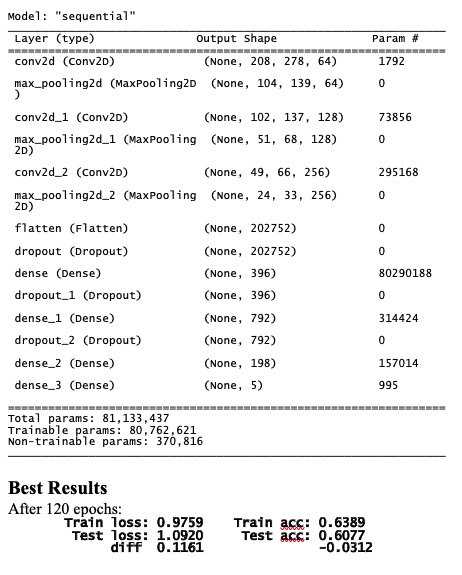
\includegraphics[scale=0.85]{Media/Layers/result.png}
\caption{Model information of the most trained and high accuracy result of the tests.}
\label{figres}
\end{figure}


\subsection{Layers \& Filters}

In order to attempt to optimize the structure and hyper-parameters of the model I took a reduced data set to run short tests on with few epochs. This reduced data set consisted of 400 of each class from the ~1500 in the data set and as such would have a very limited ceiling for accuracy on the test data but by comparing these results for test accuracy it was hoped some information could be gleaned about how to structure the model and it’s hyper-parameters for use on a larger data et. The first Parameter to decide on is the batch size, as a reasonable trade-off between accuracy and speed needs to be found to test the other parameters in a timely manner. The “starting point” model consisted of a sequential model with a re-scaling layer first to change the RGB values from -256 to 0-1 to work better with the model, then a convolutional layer with 32 filters, a pooling layer, a second convolutional layer with 64 filters, a second pooling layer, a flattening layer and then 2 dense layers. \\

Both pooling layers used 2x2 pooling with a stride of 2 and both convolutional layers used the relu activation function and a stride of 1. The first Dense layer used the “relu” activation function and the second the “softmax” function. The Loss function used was sparse categorical crossentropy with the adam optimizer. Note that all these results show the model overfitting within the 5 epochs. On the full data set, it is likely that more than 5 epochs would be required to achieve good accuracy with the sufficient data available, but as 5 epochs are sufficient for the validation accuracy to converge to an approximate point, it serves well enough for this purpose. 16 was chosen as a starting point for the batch testing as the training:testing split is 80:20 so the training data is 1600 images, a simple 100 batches per epoch. From the data, it is evident that smaller batch sizes than 16 significantly slow down processing but any positive change to the validation (or training) accuracy is minimal. \\

Larger batch size values result in a minor speed increase and a minor accuracy decrease, but it is predicted that this minor decrease is only due to the small size of data used and the negative effect on accuracy would be amplified by using this larger batch size on the full data (as evidenced by the lower training accuracy compared to smaller batch sizes), as a result a batch size of 16 was chosen and used for future tests. All of these tests also show the expect result that validation accuracy is never very high, with 20\% being as good as guessing, the model never progresses past approximately 30\%. This is can be attributed to a lack of optimisation in part but also the simple lack of data. With this value found, I then attempted to optimize the parameters of the layers, first by changing the number of filters used by the convolutional layers. \\


\begin{figure}[H]
\centering
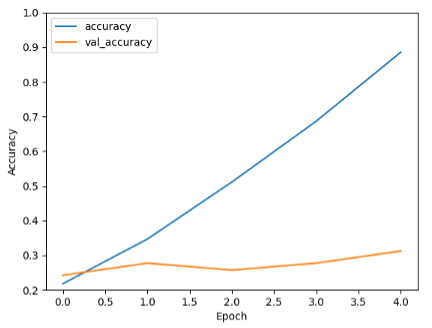
\includegraphics[scale=1.0]{Media/Testing/fig4.png}
\caption{Batch Size =32, taking ~31 seconds per epoch.}
\label{fig4}
\end{figure}

\cref{fig4} shows with 32,64 (for the first and second layers respectively) \cref{fig5} 64,128 and \cref{fig6} 16,32. While doubling the filters increased the training accuracy, it had no positive effect on the validation accuracy and made the model take far longer, so is not useful.While halving the filters had the expected effect of decreasing time per epoch, it also had the unexpected effect of increasing validation accuracy significantly (baring in mind that due to limited data to achieve speed in testing there is a cap on how much accuracy can be achieved with any model) with a peak (though not end due to overfitting) accuracy on 39.75\%. \\


\begin{figure}[H]
\centering
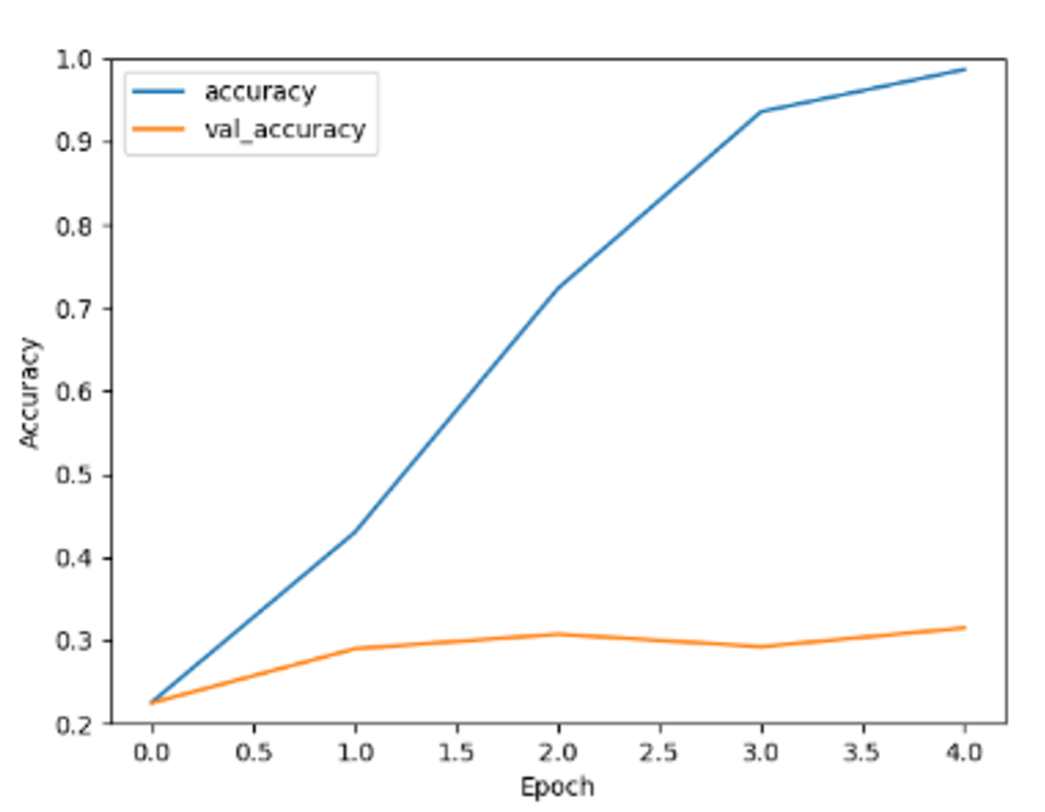
\includegraphics[scale=1.0]{Media/Testing/fig8.png}
\caption{16,64 Filters. Taking 25 seconds per epoch.}
\label{fig8}
\end{figure}

A further decrease to 12/24 Filters however did not result in more accuracy to I then removed to changing the number of filters individually rather than both at once from the 16/32 that had given the best result so far. 16/64, 16/48 and 16/16 all proved not to increase validation accuracy however, with peaks of 31.5\% ,35.75\% and 32.75\% none beat 16/32. This configuration was then tested on the full data set for 5 epochs to get some approximation of it’s actual usefulness. This still results in low validation accuracy (34.06\%) so I attempted to modify the filters on the full data set as random variance may of accounted for “improvements” on the reduced data set, getting better results with 12/24 though also getting a bizarre result where the validation accuracy starts at it’s peak and only decreases with further epochs as the training accuracy increases. \\

\begin{figure}[H]
\centering
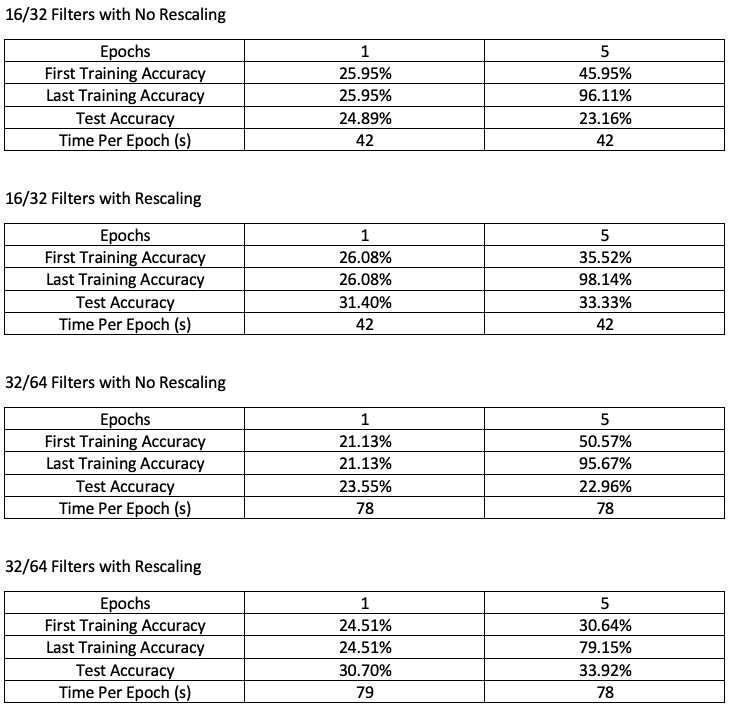
\includegraphics[scale=0.6]{Media/Layers/1.png}
\end{figure}

While previous tests had all been done with a re-scaling layer, it was worth investigating whether this layer was useful or not, and so the following results were gathered. These results show that adding a re-scaling layer has no noticeable impact on epoch time but seems to increase test accuracy significantly for no downside, so previous assumptions about using the re-scaling layer were correct to do so. The increased first training accuracy on the 5-epoch is because this is done on the model having already one 1 epoch and so this is effectively a 2nd to 6th epoch not a 1st to 5th epoch hence the increased training accuracy initially, not caused by re-scaling. \\

\begin{figure}[H]
\centering
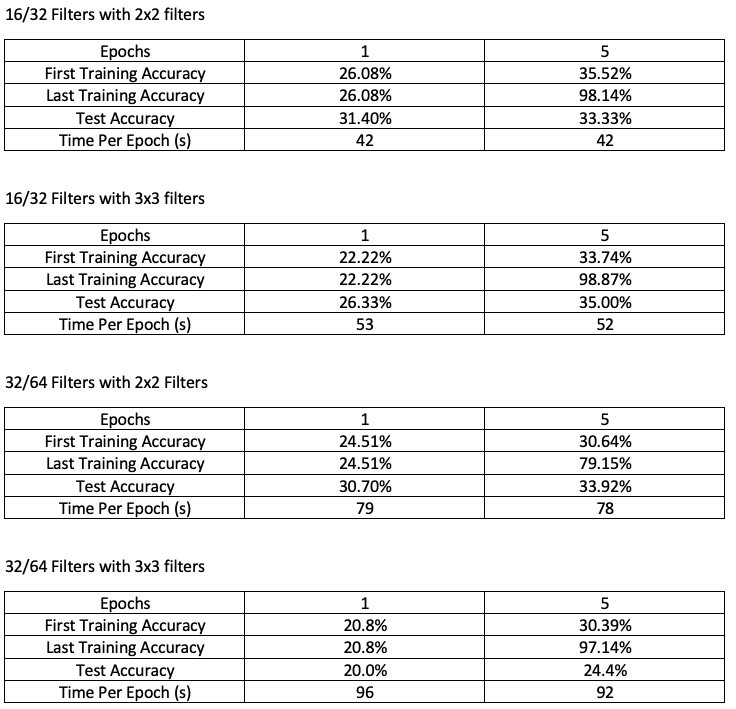
\includegraphics[scale=0.6]{Media/Layers/2.png}
\end{figure}

We then attempted to see if using larger filters of 3x3 instead of 2x2 would help test accuracy giving the results above. This resulted in a noticeable drop in accuracy for the 32/64 filter set and a marginal increase in the 16/32 filter set but this could simply be random variance at work and as it increased epoch time 2x2 filters seem preferable in this current combination of parameters. \\

\begin{figure}[H]
\centering
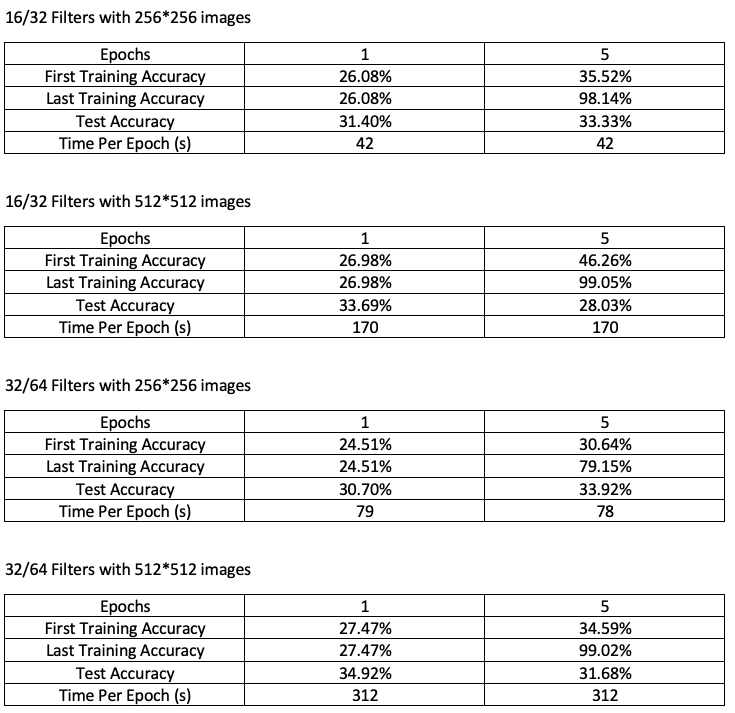
\includegraphics[scale=0.6]{Media/Layers/3.png}
\end{figure}

Using the 512x512 Images as inputs drastically increased epoch time and increased both initial and final training accuracy, however test accuracy was actually effected negatively. While the decrease in test accuracy could be due to variance even if this is the case it does not grant any increase in test accuracy for a very large increase in epoch time so the usage of 512x512 images is not useful with this current parameter combination though it could result in increased accuracy under other circumstances. \\

\subsection{Accuracy against Epochs}

Once the pre-processing was complete we could move onto modelling, once we got the first basic model working we could begin collecting data but we found that whilst the training accuracy would be very high the testing accuracy would not. The format of these models was two 2D convolution layers with max pooling between, followed by another max pooling layer which was flattened then lead into a large dense layer followed by a final dense layer with 5 classifications with a softmax activation. The default activation for the rest of the model was relu and the pool sizes were (2,2). \\

This model was tested in various ways, the first of course was adjusting the epochs to see what difference that would make. Moving from 1 epoch to 5 had a slight difference in the testing accuracy but from 5 to 15 had a slight decrease of 0.2\%. \\

\begin{table}[H]
\begin{center}
 \footnotesize
 \begin{tabular}{|c||c|c|c|}
 \hline
 \multicolumn{4}{|c|}{Accuracy against number of epochs.} \\
 \hline
 Epochs & 1 & 5 & 15 \\
 \hline \hline
 First Training Accuracy & 0.21314433217048645 & 0.21262887120246887 & 0.8505154848098755 \\
 \hline
 Last Training Accuracy & 0.21314433217048645 & 0.8141752481460571 & 0.9317010045051575 \\
 \hline
 Testing Accuracy & 0.21467182040214539	& 0.23320463299751282	& 0.23140282928943634 \\
 \hline
 \end{tabular} \\
\end{center}
\end{table}

You can see that more than 1 epoch is clearly favourable however none of the results were ideal with barely a 25\% accuracy it may as well be luck that is driving the process. It seems that the model was being heavily overfitted as towards the end of the 15-epoch run all the training accuracies were very close with a range of 2\%. This same test of epochs making a difference was done with 2 other models also, one model with double the number of filters in the convolutional layers and one with the sigmoid activation function instead of the relu function. The results were as follows. \\

\begin{table}[H]
\begin{center}
 \footnotesize
 \begin{tabular}{|c||c|c|c|}
 \hline
 \multicolumn{4}{|c|}{Accuracy against number of epochs with double filters.} \\
 \hline
 Epochs & 1 & 5 & 15 \\
 \hline \hline
 First Training Accuracy & 0.21546392142772675 &	0.2033505141735077 & 0.7097938060760498 \\
 \hline
 Last Training Accuracy & 0.21546392142772675 &	0.6847938299179077 & 0.8432989716529846 \\
 \hline
 Testing Accuracy & 0.21441441774368286	& 0.22651222348213196	& 0.22857142984867096 \\
 \hline
 \end{tabular} \\
\end{center}
\end{table}

\begin{table}[H]
\begin{center}
 \footnotesize
 \begin{tabular}{|c||c|c|c|}
 \hline
 \multicolumn{4}{|c|}{Accuracy against number of epochs using the Sigmoid function.} \\
 \hline
 Epochs & 1 & 5 & 15 \\
 \hline \hline
 First Training Accuracy & 0.20463918149471283 & 0.20412370562553406	& 0.20721650123596191 \\
 \hline
 Last Training Accuracy & 0.20463918149471283 &	0.20721650123596191 & 0.2033505141735077 \\
 \hline
 Testing Accuracy & 0.20000000298023224	& 0.20000000298023224 & 0.20000000298023224 \\
 \hline
 \end{tabular} \\
\end{center}
\end{table}

The double filters did look promising with the gradual increase in training accuracy, I was hoping that the model would not end up over fitting but it still resulted in a 23\% accuracy for the testing set. The sigmoid function however seemed to be a complete failure for this set, the accuracy for the training and testing did not change throughout with no difference when increasing the number of epochs either. I would have liked to test the epochs further however with 15 epochs difference granting an increase of 0.0025\% the number of epochs would have been massive, especially with a processing time of a minute an epoch. So far, all models have been completed without a validation set, this was changed for the next model as we wanted to test what difference this could make for the training and validation accuracy compared to the testing accuracy at the end. \\

\begin{table}[H]
\begin{center}
 \footnotesize
 \begin{tabular}{|c||c|c|c|}
 \hline
 Epochs & 1 & 5 & 15 \\
 \hline \hline
 First Training Accuracy & 0.2177537977695465 &	0.5139774680137634 &	0.975968599319458 \\
 \hline
 Last Training Accuracy & 0.2177537977695465 &	0.9565963745117188 &	0.9855321049690247 \\
 \hline
 First Validation Accuracy & 0.21121923625469208 &	0.23125357925891876 &	0.22839152812957764 \\
 \hline
 Last Validation Accuracy & 0.21121923625469208 &	0.24327418208122253	& 0.23526044189929962 \\
 \hline
 Testing Accuracy & 0.2319587618112564 &	0.20000000298023224 &	0.223195880651474 \\
 \hline
 \end{tabular} \\
\end{center}
\end{table}

Even with validation data there was not a change in the result for the testing. The split for validation was 70/30 here with similar results found at 80/20. An issue that might be causing this could be the split for training and testing data as a whole, so far the split has been 50/50 which could be far too few images for the model to correctly learn. Having more could prevent overfitting and allow for better performance in the testing data set, so the next thing we tried was a 75/25\% split for training/testing respectively. This change alone caused negligible changes to the accuracy for training validation and testing however changing the way that the data was input did have a small positive change to the testing accuracy. Normalising the rgb values input into the model by dividing by 255 caused an increase to 30\% testing accuracy after 15 epochs, this was by far the highest testing value achieved yet so suggests it is on the right line by doing so. The values for this are as follows. \\

\begin{table}[H]
\begin{center}
 \footnotesize
 \begin{tabular}{|c||c|c|c|}
 \hline
 Epochs & 15 \\
 \hline \hline
 First Training Accuracy & 0.2457086741924286 \\
 \hline
 Last Training Accuracy & 0.9995095729827881 \\
 \hline
 First Validation Accuracy & 0.282198041677475 \\
 \hline
 Last Validation Accuracy & 0.29421865940093994 \\
 \hline
 Testing Accuracy & 0.2994845509529114 \\
 \hline
 \end{tabular} \\
\end{center}
\end{table}

After getting a better results from normalising the data we thought to try some different models and to adjust the size of the images from data set, changing the model on its own had lower accuracy than above however by adjusting the image width/height to 224 (as seen elsewhere to be quite common). we also let this model run for 30 epochs as the accuracy's were still gently increasing past 15 and began to plateau around 30 so this is where we took measurements. \\

\begin{table}[H]
\begin{center}
 \footnotesize
 \begin{tabular}{|c||c|c|c|}
 \hline
 Epochs & 30 \\
 \hline \hline
 First Training Accuracy & 0.20042918622493744 \\
 \hline
 Last Training Accuracy & 0.9399141669273376 \\
 \hline
 First Validation Accuracy & 0.17768239974975586 \\
 \hline
 Last Validation Accuracy & 0.3579399287700653 \\
 \hline
 Testing Accuracy & 0.38092783093452454 \\
 \hline
 \end{tabular} \\
\end{center}
\end{table}

This yielded the highest testing accuracy so far with 38\%. For now we will keep the image size as set here and will continue to adjusting the models to see what impact this will have on the results. The next model we tried was much larger and also included data augmentation which would rotate the images randomly also, this was giving promising results with a peak validation accuracy of 60\%, this was on an upward trend however so the validation could have become stable at 60\% should this have been left for longer. \\

\begin{figure}[H]
\centering
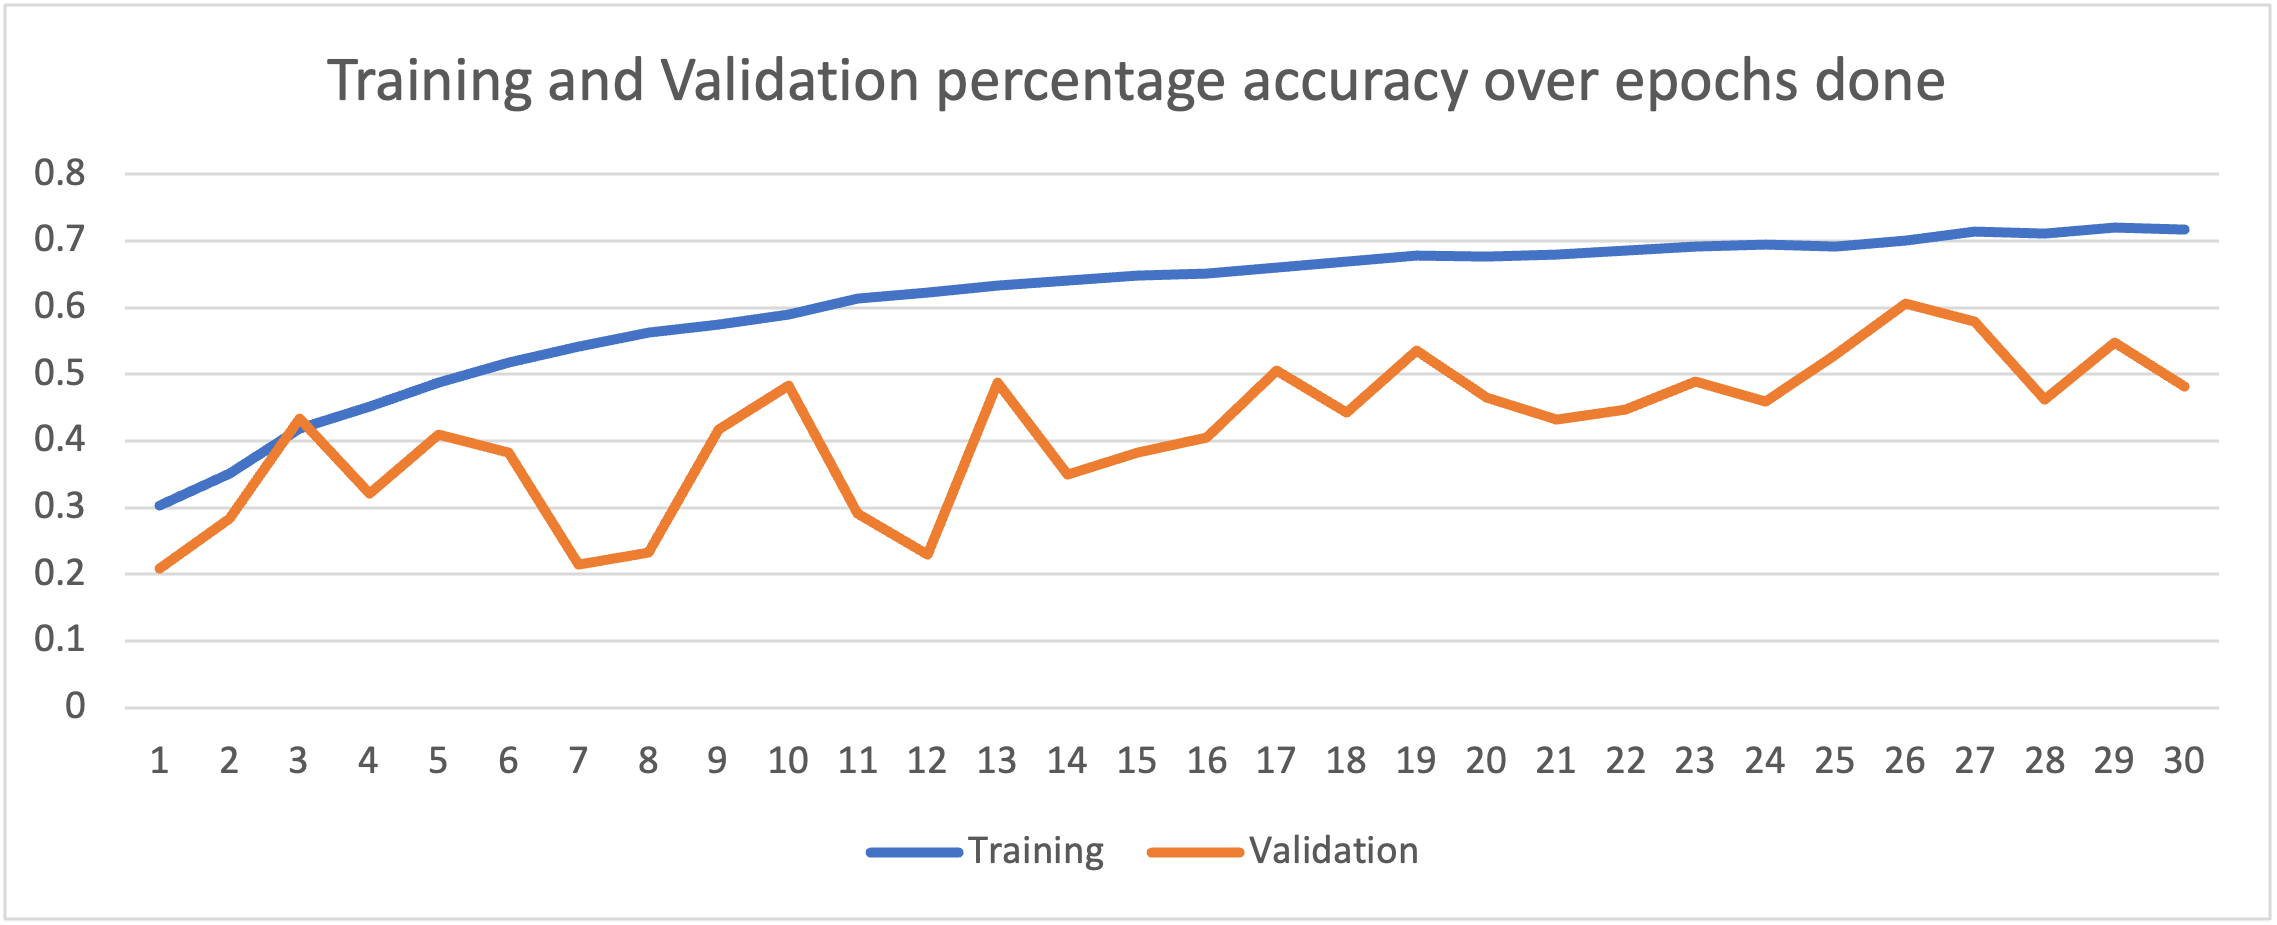
\includegraphics[scale=0.85]{Media/Vali/val1.png}
\caption{Accuracy of the training and validation data undertaking 30 epoch cycles.}
\label{figva1}
\end{figure}

The testing accuracy for this model was 47\% which is very close to the validation so if we had stopped the model on that peak it could have performed much better. Since the training accuracy was slowly increasing we felt that there could be more that the model could learn so after continuing the model for between 5-15 epochs at a time it still showed no sign of slowing down with a validation accuracy of 63\% and testing of 65\% at 85 epochs. Continuing further to 100 continue to show the upward trend of the training accuracy however the validation became more erratic in its changes and on the 100th epoch when testing was done it resulted in an accuracy of 50\%, far lower than before. \\

\begin{figure}[H]
\centering
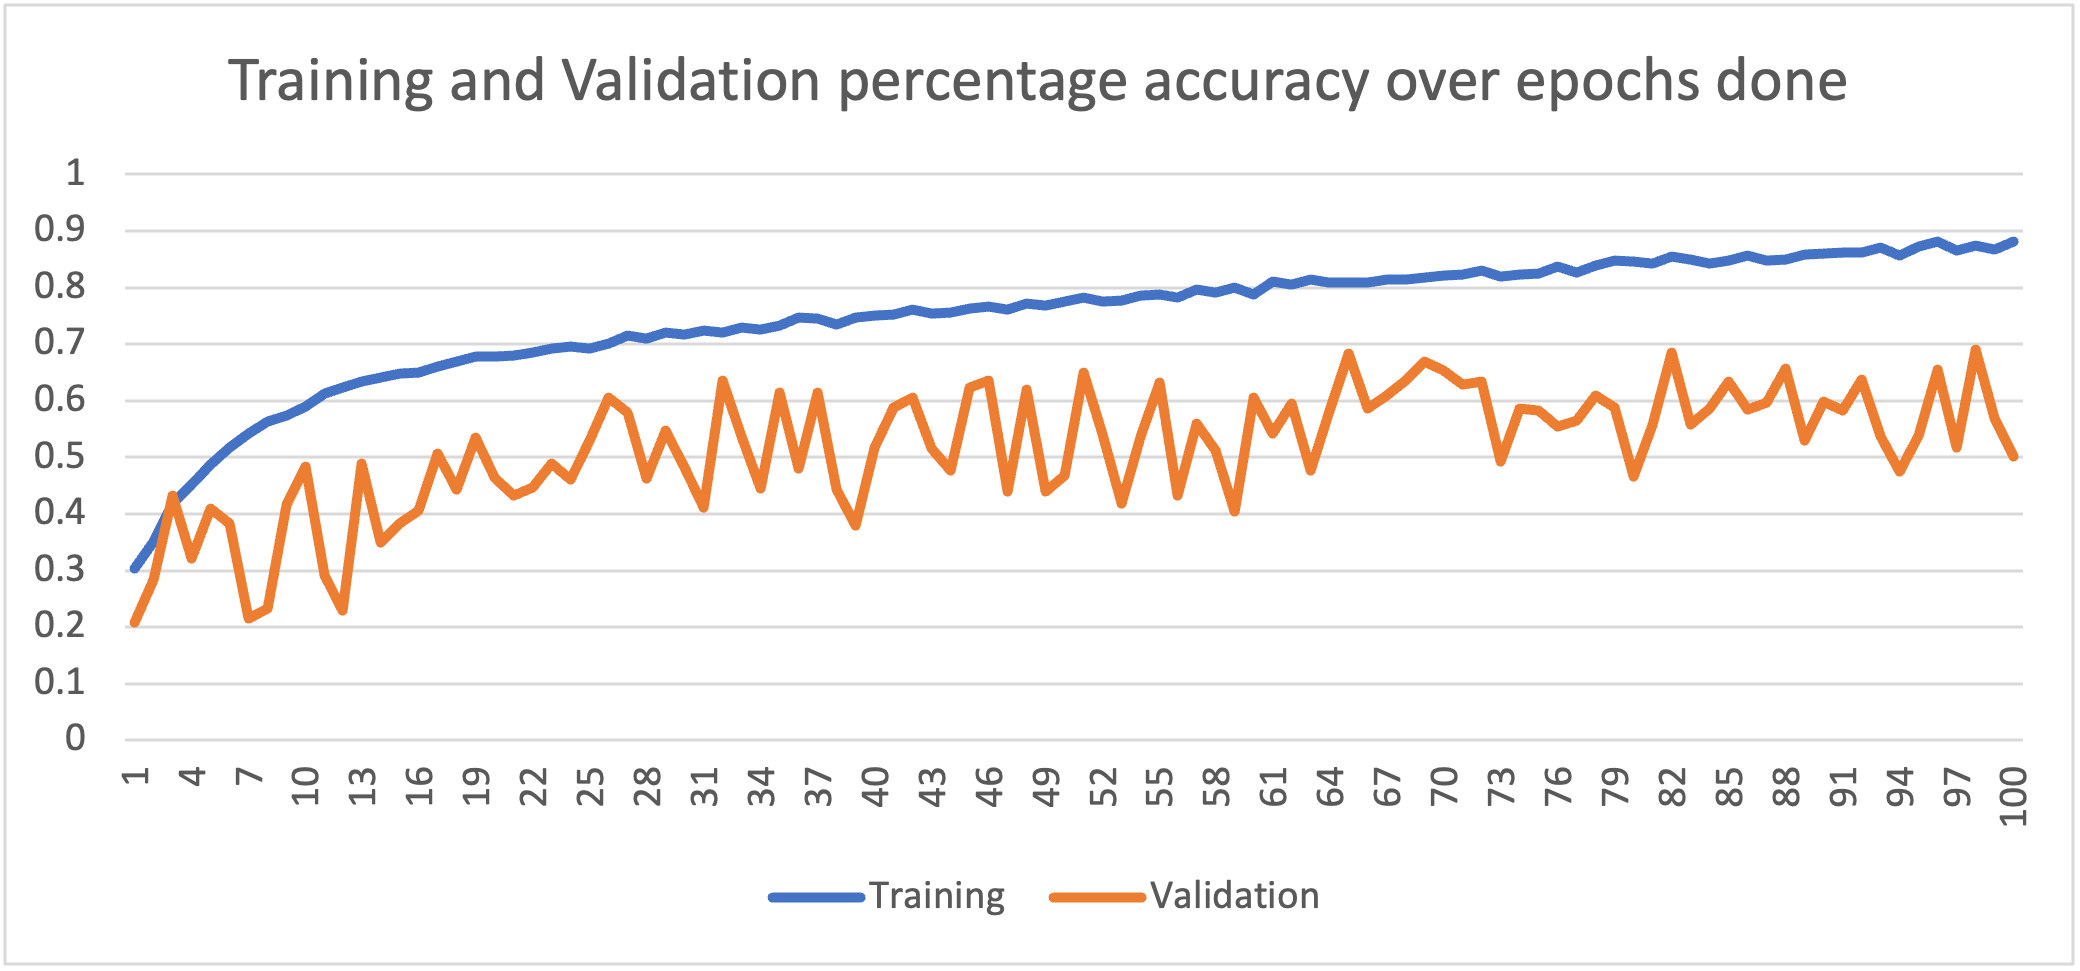
\includegraphics[scale=0.95]{Media/Vali/val2.png}
\caption{Accuracy of the training and validation data undertaking 100 epoch cycles.}
\label{figval2}
\end{figure}

Once again the testing was done on a dip so it is likely by running single epochs on the same model at this point could give a good model with high accuracy for validation. When running the model for single epochs at 101 there was a validation accuracy of 64\% and a testing accuracy of 67\%, at 102 the validation accuracy went to 65\% and the testing accuracy remained at 67\%. 103 and 104 began to dip again giving accuracy's of around 62\% however they are all beginning to remain consistently above 60\% which was very promising until at 105 when it dipped to 51\%. Running continuously now it was clear that it had peaked and was likely to not rise again. 
